%----------------------------------------------------------------------------------------
\documentclass[paper=letter, fontsize=11pt]{article}
\usepackage[english]{babel} % English language/hyphenation
\usepackage{amsmath,amsfonts,amsthm} % Math packages
\usepackage[utf8]{inputenc}
\usepackage{float}
\usepackage{lipsum} % Package to generate dummy text throughout this template
\usepackage{blindtext}
\usepackage{graphicx} 
\usepackage{pgfgantt}
\usepackage{fourier}
\usepackage{pdfpages}
\usepackage{caption}
\usepackage{subcaption}
\usepackage[sc]{mathpazo} % Use the Palatino font
\usepackage[T1]{fontenc} % Use 8-bit encoding that has 256 glyphs
\linespread{1.05} % Line spacing - Palatino needs more space between lines
\usepackage{microtype} % Slightly tweak font spacing for aesthetics
\usepackage[hmarginratio=1:1,top=32mm,columnsep=20pt]{geometry} % Document margins
\usepackage{multicol} % Used for the two-column layout of the document
%\usepackage[hang, small,labelfont=bf,up,textfont=it,up]{caption} % Custom captions under/above floats in tables or figures
\usepackage{booktabs} % Horizontal rules in tables
\usepackage{float} % Required for tables and figures in the multi-column environment - they need to be placed in specific locations with the [H] (e.g. \begin{table}[H])
\usepackage{hyperref} % For hyperlinks in the PDF
\usepackage{lettrine} % The lettrine is the first enlarged letter at the beginning of the text
\usepackage{paralist} % Used for the compactitem environment which makes bullet points with less space between them
\usepackage{abstract} % Allows abstract customization
\usepackage[round]{natbib}
\renewcommand{\abstractnamefont}{\normalfont\bfseries} % Set the "Abstract" text to bold
\renewcommand{\abstracttextfont}{\normalfont\small\itshape} % Set the abstract itself to small italic text
\usepackage{titlesec} % Allows customization of titles

\renewcommand\thesection{\Roman{section}} % Roman numerals for the sections
\renewcommand\thesubsection{\Roman{subsection}} % Roman numerals for subsections

\titleformat{\section}[block]{\raggedright\large}{\thesection.}{1em}{} % Change the look of the section titles
\titleformat{\subsection}[block]{\raggedright\large}{\thesubsection.}{1em}{} % Change the look of the section titles
\newcommand{\horrule}[1]{\rule{\linewidth}{#1}} % Create horizontal rule command with 1 argument of height
\usepackage{fancyhdr} % Headers and footers
\pagestyle{fancy} % All pages have headers and footers
\fancyhead{} % Blank out the default header
\fancyfoot{} % Blank out the default footer

\fancyhead[L]{Manifold Dynamics and their Applications to Low-Energy Transfers -- PPR}
\fancyfoot[RO,LE]{\thepage} % Custom footer text
\usepackage{fourier}
	\usepackage{listings}

%----------------------------------------------------------------------------------------
%       TITLE SECTION
%----------------------------------------------------------------------------------------
\title{\vspace{-15mm}\raggedright\fontsize{18pt}{10pt}\selectfont\textbf{Manifold Dynamics and their Applications to Low-Energy Transfers: Project Plan Report}} % Article title
%\raggedright\author{
%\large%\raggedright
%{\raggedright Jack Tyler}\\[2mm]
%%\thanks{A thank you or further information}\\ % Your name
%%\normalsize \href{mailto:marco.torres.810@gmail.com}{marco.torres.810@gmail.com}\\[2mm] % Your email address
%}
\date{}

%----------------------------------------------------------------------------------------
\begin{document}
\maketitle % Insert title
%\thispagestyle{fancy} % All pages have headers and footers

\section*{Project Overview}
Manifold Dynamics and their Applications to Low-Energy Transfers aims to study the dynamical phenomena of the circular-restricted three-body problem (CR3BP): an examination of the motion of a third, massless particle moving under the influence of two other particles (primaries) that orbit in circles about their barycenter. In particular, the CR3BP yields many dynamical structures -- stable and unstable manifolds and bouding surfaces -- that provide means for matter transfer into and from the primaries. Exploiting these dynamical phenomena can provide the construction of complex, non-Keplerian orbits to achieve mission objectives, as well as potential propellant savings \citep{Parker2014}. 

Its' inception is believed to have begun with \citep{Euler1736}, who introduced a synodic coordinate system during his studies of Lunar motion. Attracting a range of well-known mathematicians to its' formulation, the three-body problem received significant contributions from \citep{Lagrange}, who discovered some of the equilibrium solutions now known as the Lagrangian points, and \citep{Jacobi1829} who `re-discovered' the Jacobi integral, the only constant of motion in the CR3BP. \citep{Hill1906} later used this integral in his formulation of forbidden regions and bounded motion. Perhaps most important for analysis of the CR3BP, \citep{Poincare1899}'s methods of section, phase-space and deterministic chaos ended the classical period of study for the three-body problem \footnote{For the development of these methods, Sweden's King Oscar II awarded Poincar\'e a prize to award him for being the first to solve the n-body problem. Poincar\'e had not, in fact, even solved the general case of the three-body problem.}\citep{theoryoforbits}.

The use of this formulation of spacecraft motion was first used to construct a low-energy transfer by Edward Belbruno, to rescue the Japanese MUSES-A mission -- now renamed Hiten -- and place it into a Lunar orbit \citep{Belbruno2004}. Since then, the CR3BP has been studied heavily for its' ability to reveal mission plans about the Lagrangian points -- now home to several scientific payloads -- and dynamically-assisted trajectories, including those used by spacecraft such as SMART-1, Genesis, and GRAIL \citep{Topputo2005}. 

By studying the equations of motion of the CR3BP (Equations \ref{eq:governingeqs} through 4), along with a numerical computation suite, the construction and visualisation of these orbits is possible. Figure \ref{f:lyapunov} reports a family of periodic Lyapunov -- planar -- orbits about a Lagrangian point, constructed utilising a software suite in MATLAB, and a numerical technique known as differential correction.

\begin{align}\label{eq:governingeqs}
\ddot{x} - 2\dot{y} = \frac{\partial \Omega}{\partial x} \\
\ddot{y} + 2\dot{x} = \frac{\partial \Omega}{\partial y} \\
\ddot{z} = \frac{\partial \Omega}{\partial z}\\
\Omega = \frac{1}{2} (x^2 + y^2) + \frac{1 - \mu}{r_{12}} + \frac{\mu}{r_{23}}
\end{align}


By determining and applying disturbances to these orbits in their stable and unstable directions, and integrating the equations of motion forwards or backwards, we discover trajectories that exponentially approach or depart these periodic orbits. Discretizing and plotting these trajectories around the entirety of the orbit yields stable and unstable manifold tubes, respectively. It is these which are used to construct `low-energy' transfers\footnote{The definition of low-energy is ambiguous. For this case, low-energy is taken to represent a transfer that exploits natural and/or dynamical phenomena to reduce spacecraft propellant usage.}; these manifolds are visualised in Figure \ref{f:manifolds}.

Multiple uses for these missions have been proposed: \citep{Sanchez2016} has proposed their usage for asteroid retrieval missions, where the required impulse to capture is significantly reduced when utilising stable manifolds. Alternatively, \citep{Belbruno1993} and \citep{Luo2015} recommended them for use in interplanetary transfers, where the stable manifold acts as a route for quasi-ballistic capture, decreasing delta-V requirements in some cases, and increasing the launch periods. These uses will be evaluated in a full, sample mission case study to form the main deliverable for the project.

\begin{figure}
\centering
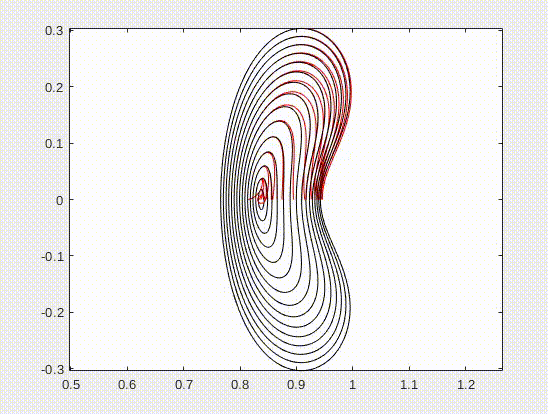
\includegraphics[height=.25\textheight]{../presentation/gif/manifolds-330}
\caption{A family of Lyapunov orbits about Earth-Moon L$_1$ ($\mu = 0.0121$). The red lines indicate the interations of the differential correction subroutines.}
\label{f:lyapunov}
\end{figure}

\begin{figure}
\centering
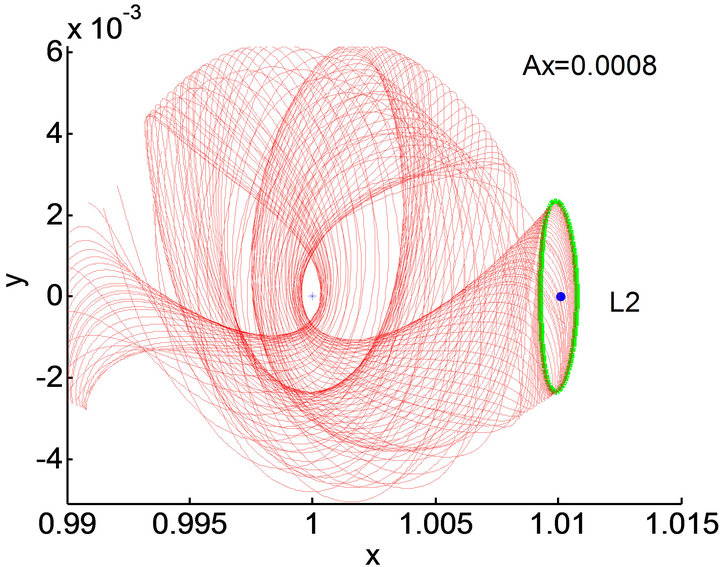
\includegraphics[height=.25\textheight]{../presentation/manifoldtubes}
	\caption{Unstable manifold computed from initial state $x_0$ using the relation $x_0\prime = x_0 \pm \varepsilon\frac{\lambda}{\lvert \lambda \rvert}$, where $\lambda$ represents the unstable eigenvalue of the Jacobian matrix of the local subspace; $\varepsilon$ = 10\textsuperscript{-6}}
\label{f:manifolds}
\end{figure}


\section*{Project Outcomes, Aims and Scope}

	The project outcome is to deliver a full case study for a mission that exploits dynamical phenomena of the CR3BP. To this end, it sets the following aims:

			\begin{itemize}
				\item A comprehensive literature review on CR3BP theory, potential applications and numerical techniques for the contruction of orbits in the CR3BP;
				\item A suitable mission selection that will exploit a range of features of the CR3BP;
				\item The creation of software bundle to allow for the computation of the mission analyses and orbit construction.
			\end{itemize}

			with the following scope of work:

	\begin{itemize}
		\item  The mathematics behind the CR3BP and its' dynamical phenomena;
		\item The theory behind, and implementation of, numerical techniques for orbit construction including numerical integration, differential correction and optimisation;
		\item Studies of mission trade-offs and requirements;
		\item Studies and implementation of software analytics: code coverage, MC/DC coverage, static/dynamic program analysis and parallel processing techniques for minimising runtimes.
	\end{itemize}


\section*{Training needs analysis}

An induction onto the Lyceum supercomputing cluster may be required, but is as yet unknown. No other training is required.

\section*{Gantt Chart}

Figure \ref{f:ganttchart} reports the provisional Gantt chart for the project.

\section*{Meeting minutes}

Meeting minutes are recorded in plain text in Vim during the meetings. They are reported here unformatted. \\[1cm]


	\resizebox{\textwidth}{!}{
	\lstinputlisting[language={}]{minutes-1.txt}
	}

	\resizebox{\textwidth}{!}{
\lstinputlisting[language={}]{minutes-2.txt}
}


\begin{figure}
	\centering
	\resizebox{\textwidth}{!}{
	\begin{ganttchart}{1}{24}
		  \gantttitle{IP provisional time plan; weeks after 03/10/17}{24} \\
		  \gantttitlelist{1,...,24}{1} \\
		 % \ganttgroup{Group 1}{1}{7} \\
		  \ganttbar{Literature review \& mission selection}{1}{9} \\
		  %\ganttlinkedbar{Mission selection}{4}{4} \ganttnewline
		  \ganttlinkedmilestone{Check required knowledge}{10-12} \ganttnewline
		  \ganttlinkedbar{Programming software suite}{14}{18}\ganttnewline
		  \ganttlinkedbar{Finalising report write-up}{18}{24}\ganttnewline
		  %\ganttlinkedk{elem2}{elem3}
		  %\ganttlink{elem3}{elem4}
	\end{ganttchart}
}
\caption{Provisional Gantt chart for the Part III individual project.}
	\label{f:ganttchart}
\end{figure}
%\begin{figure}
%	\resizebox{\textwidth}{!}{
%	\lstinputlisting[language={}]{minutes-1.txt}
%	}
%\end{figure}
%\begin{figure}
%	\resizebox{\textwidth}{!}{
%\lstinputlisting[language={}]{minutes-2.txt}
%}
%	
%	\caption{Meeting minutes for 05-10-17 and 10-10-17}
%\end{figure}
\newpage
\clearpage
\bibliographystyle{plainnat}
\bibliography{ref.bib}
%\bibliography
\newpage

\includepdf[pages={-}, width=\linewidth]{../presentation/demo.pdf}



\end{document}
